\documentclass[twoside, a4paper, leqno]{article}
\usepackage[inner=3cm, outer = 2cm, top=2cm,bottom=2.5cm]{geometry}
\usepackage[fontsize=13pt]{scrextend}

\renewcommand{\abstractname}{\large ABSTRACT\\}
\author{Hoang-Long.Vu}
\date{\today}
\title{AUDIO AMPLIFIER}

%header and footer
\usepackage{fancyhdr}
\pagestyle{fancy}
\fancyhf{}
\fancyhead[LE,RO]{Audio Amplifier}
\fancyhead[RE,LO]{Hoang-Long.Vu - 20182926}
%\fancyfoot[RE,CO]{\leftmark}
\fancyfoot[LE,RO]{\thepage}

%equation
\usepackage{siunitx}
\usepackage{mathtools, amsmath,amsxtra,amssymb,latexsym, amscd,amsthm}
\usepackage{graphicx}
\usepackage{colonequals}

%cover
\usepackage{tikz}
\usetikzlibrary{calc}
\usepackage{indentfirst}
\usepackage{titlesec}
\usepackage{tabularx}
\usepackage{float}

%link
\usepackage{hyperref}

\begin{document}
	\begin{titlepage}
\begin{tikzpicture}[overlay,remember picture]
\draw [line width=3pt]
    ($ (current page.north west) + (3.0cm,-2.0cm) $)
    rectangle
    ($ (current page.south east) + (-2.0cm,2.5cm) $);
\draw [line width=0.5pt]
    ($ (current page.north west) + (3.1cm,-2.1cm) $)
    rectangle
    ($ (current page.south east) + (-2.1cm,2.6cm) $); 
\end{tikzpicture}
\begin{center}
\vspace{-12pt}  HANOI UNIVERSITY OF SCIENCE AND TECHNOLOGY \\
\textbf{\fontsize{13pt}{0pt}\selectfont SCHOOL OF ELECTRONICS AND TELECOMMUNICATION}
\vspace{0.5cm}
 \begin{figure}[H]
     \centering
     \includegraphics[width=1.53cm,height=2.26cm]{figure/logodhbk.png}
 \end{figure}
\vspace{1.5cm}
\fontsize{24pt}{0pt}\selectfont FINAL PROJECT\\
\vspace{12pt}
\textbf{\fontsize{32pt}{0pt}\selectfont ELECTRONIC CIRCUIT I}
\vspace{1.5cm}
\end{center}
\hspace{6pt}\textbf{\fontsize{14pt}{0pt}\selectfont Topic:}
\begin{center}
    \textbf{\fontsize{20pt}{0pt}\selectfont AUDIO AMPLIFIER}\\

\vspace{1.5cm}
\begin{table}[H]
    \centering
    \begin{tabular}{l l}
 \fontsize{14pt}{0pt}\selectfont Student:    & \fontsize{14pt}{0pt}\selectfont VU HOANG LONG - 20182926 \vspace{6pt} \\ 
     &\fontsize{14pt}{0pt}\selectfont class CTTT Dien tu 01 - K63 \vspace{6pt}\\
\fontsize{14pt}{0pt}\selectfont Instructor: & \fontsize{14pt}{0pt}\selectfont DR. NGUYEN VU THANG
\end{tabular}
\end{table}
\vspace{3.5cm}
 \fontsize{14pt}{0pt}\selectfont Hanoi, \today
\end{center}
\end{titlepage}
\cleardoublepage

	\maketitle
	
	\newpage
	\section*{ \textbf{List of Abbreviation and Symbols}}
	\begin{itemize}
		\item \textbf{KVL}: Kirchhoff's Voltage Law
		\item \textbf{KCL}: Kirchhoff's Current Law
		\item \textbf{AC}: Alternating Current
		\item \textbf{DC}: Direct Current
		\item \textbf{P}: Power
		\item \textbf{V}: Voltage
		\item \textbf{I}: Current
		\item \textbf{R}: Resistance
		\item \textbf{C}: Capacitance
		\item \textbf{f}: Frequency
		\item \textbf{$\beta$}: gain coefficient
		\item \textbf{Z}: Impedance
		\item \textbf{RMS}: Root Mean Square
		\item \textbf{p-p} peak-to-peak
		
	\end{itemize}
		
	\newpage
	\listoffigures
	\newpage
	\tableofcontents
	\newpage
	\begin{abstract}
		Electronic Circuit is an essential subject for every Electronics and Telecommunications Engineering student. This subject covers a huge amount of knowledge about electronic devices and circuit theory, help students to profoundly understand the fountain of the related concepts, also how to apply them to the real life. Accordingly, to have a general look of what we have learned, I try to do a project about making \textit{An Audio Amplifier}. 
		
		Within five parts, this report covers the entire process I have followed to accomplish my final product. In the first part \textbf{\textit{Introduction}}, I will describe in details the specification of my amplifier, also its internal structure and features. The second part \textbf{\textit{Calculation and Simulation}} will reveal the way how I got the specific values for each individual parameters, also the schematic design of my circuit through each stage, then cover up by the simulation. To manufacture the product, I have to make its PCB Design, and this step will be introduced in \textbf{\textit{Part III: PCB Design}}. The last part \textbf{\textit{Making Product and Testing}} will finish the whole procedure by comparing the practical measured parameters with the theoretical calculated ones.
		
		Throughout this project, I have found my happiness of the first productive circuit I have ever made. Thanks to it, I also understand more about what you have taught us. Anyway, due to the first time I make a multi-stage circuit myself, my product maybe not the well-being one, even sometimes I stuck in difficulties. Nevertheless, it is very kind of you that you are always ready to help me overcome those drawbacks and accomplish my achievement.
		
 		\raggedleft \textit{Sincerely,}
		\\ \raggedleft \textit{Long.}
	\end{abstract}
	
	\newpage
	\part{Introduction}
	\section{Description}
		\begin{itemize}
			\item An audio amplifier is a device or a system that helps to amplify audio signals with low-power source such as output signal from smart phone's audio jack. The application of audio amplifiers can be seen everywhere, mostly in loudspeaker or music system in house club, movie theater, etc.
			\item The audio amplifier receives a very small input signal, normally measured as mili-watts (mW) and amplifies each individual parameter of the original signal through multi-stages. At the output, the obtained power is much higher than the pure one (about some watts), depends on the properties of the output speaker(s).
			\item Those parameters that will be modified (particularly amplified) are usually amplitude (Voltage), strength (Current), or power. In some complex system, also frequency could be change to shift the tone's height (deeper within lower frequency and vice versa). However, in the restriction of this project, my device only works with amplitude, intensity and power.
		\end{itemize}
		
		
	\section{Requirement}
	\subsection{Functional Requirement}
		\begin{itemize}
			\item Able to amplify the audio signal.
			\item Minimize the effects of noise, signal distortion.
			\item Compatible with variety of common sources.
			\item Working properly with 12V DC-supplier.
		\end{itemize} 
	\subsection{Non-Functional Requirement}
		\begin{itemize}
			\item Easy to use, repair and customize.
			\item Low price.
			\item Small and portable.
		\end{itemize}
	
	\section{Specification}
	\subsection{Input parameters}
		\begin{itemize}
			\item Supplier: 12V-DC.
			\item Input audio signal:
				\subitem Voltage(RMS): 10-100mV-AC.
				\subitem Frequency: 16Hz-20kHz. 
		\end{itemize}
	\subsection{Output parameters (Speaker)}
		\begin{itemize}
			\item Resistance: 4$\si{\ohm}$.
			\item Power: 3W.
			\item Voltage amplification factor:  45.
		\end{itemize}
	
	\subsection{Choosing Devices}
	In this circuit, I use 5 transistors, including 3 power transistors. The transistor for amplitude amplifying purpose named \textit{\textbf{BC547B}}, which is a very common NPN transistor type could be found in every electronic device store. BC548 one is also good, but I do not choose it due to its lower cut-off voltage, compared to the previous one. For the power transistors, \textit{\textbf{TIP41C}} and \textit{\textbf{TIP42C}} are good choices, where TIP41C is NPN transistor type, TIP42C is PNP one.
	
	All the installed capacitors are biased capacitors, which ranged from $220\si{\micro}F$ to $2.2\si{\milli} F$ (depending on the formula $C = \frac{1}{2\pi f Z_c}$, where $f \approx 16Hz$ - \textit{the minimum listening level of humans} $Z_C = Z_{i/o}$), are used for restricting the DC current.
	
	\section{Block Diagram}
		\begin{center}
			\begin{figure}[htp]
				\begin{center}
					\includegraphics[scale = .45]{figure/blockdiagram.png}
				\end{center}
				\caption{System Block Diagram}
				\label{refFigure1}
			\end{figure}
		\end{center}
	
	\newpage
	\part{Calculation and Simulation}
	\section{Calculation}
		For the suitable design purpose, I choose the voltage divider configuration for the first stage, the next stage will base on the Emitter Follower Darlington connection, and the last will be applied the AB class power amplifier configuration.
		
		Accordingly, the first configuration have large voltage amplification coefficient, meanwhile the remained ones have the voltage amplification factor approximate one.
		
		Following the requirement, the system has the input voltage from $10mV$ to $100mV$, while the output speaker has the resistance of $4\si{\ohm}$ and power of $3W$. Consequently, I obtain the maximum amplitude amplification factor so that the system works properly:
		
		\textit{First, I calculate the maximum can-be-reached AC output voltage applied on the speaker:}
		\begin{align}
			V_{o_{max}}(p) = \sqrt{2PR} = \sqrt{2(3W)(4\si{\ohm})} \approx 4.9V
		\end{align}
	
		\textit{Within the input voltage of maximum $100mV$, I obtain the maximum voltage amplification factor of the entire circuit:}
		\begin{align}
			A_{v_{max}} = \frac{Vo_{max}}{Vi_{max}} = \frac{4.9V}{100mV} \approx 49
		\end{align}
		
		\textit{Hence we choose the maximum can-be-reached voltage amplification factor of $49$}.
		
		Anyway, for safe working purpose, I choose the gain of the first stage of slightly less than the absolution of $-45$ (by round up the bias resistance in the below calculation, negative sign due to the specification of voltage divider configuration, that cause the phase reverse of the signal but not affects the sound's quality), while the other ones have the gain approximate one, so that the entire absolute gain of the system close to $45$ as requirement.
		
		For whom want to know why I choose the value $12V$ for the supplier, this value has obtained from the maximum required AC output voltage applied on the speaker as mentioned above:
		\begin{align}
			V_{o_{max}}(p-p) = 2\sqrt{2}\times V_{o_{max}}(rms) = 2\sqrt{2}\times 3.46V \approx 9.79V
		\end{align}
	
		$\Leftrightarrow$ Choose \fbox{$V_{supplier} = 12V$}.
		
		To make sure that the entire circuit works properly throughout all the stages, I choose the voltage difference between the emitter and collector (denoted as $V_{CE}$) of every transistor equals to six volts ($V_{CE} = 6V$), which is a half of the power supplier's voltage. At this point, I ensure that the range of AC signal's amplitude that the signal is transmitted without distortion reaches the maximum value.
		
	\subsection{Stage 1: Pre-Amplifier}
		\subsubsection*{Choosing the Q-Point}
		Base on BC547B's datasheet, I choose the working point of this transistor: 
		\begin{itemize}
			\item CE-voltage difference: $V_{CEQ1} = 6V$.
			\item Base current: $I_{BQ1} = 50\si{\micro}A$.
			\item Collector current: $I_{CQ1} = 12\si{\milli}A$.
			\item Amplification Factor: $\beta = \frac{I_{CQ1}}{I_{BQ1}} = 240$.
		\end{itemize}		
		
		\begin{center}
			\begin{figure}[htp]
				\begin{center}
					\includegraphics[scale = .8]{figure/Q_point_BC547B.png}
				\end{center}
				\caption{BC547B's Characteristic Line}
				\label{refFigure2}
			\end{figure}
		\end{center}
	
		\subsection*{Calculating}
		
		\begin{center}
			\begin{figure}[htp]
				\begin{center}
					\includegraphics[scale = .6]{figure/Stage1.png}
				\end{center}
				\caption{Stage 1: Pre-Amplifier}
				\label{refFigure3}
			\end{figure}
		\end{center}
		
		\subsubsection*{DC-mode parameters}
		\begin{itemize}
			\item Calculate Emitter Resistance $R_{EQ1}$
				Emitter Current: $I_{EQ1} = \frac{\beta+1}{\beta}\times I_{CQ1} = \frac{240+1}{241}\times12\si{\milli}A \approx 12\si{\milli}A$
			
				Choosing $V_{EQ1} = \frac{V_{CC}}{10} = 1.2V \Leftrightarrow R_4 + R_5 = R_{EQ1} = \frac{V_{EQ1}}{I_{EQ1}} = \frac{1.2V}{12\si{\milli}A} = 100\si{\ohm}$
				
				\fbox{$R_4 + R_5 = R_{EQ1} = 100\si{\ohm}$}
				
			\item Calculate Collector Resistance $R_{CQ1}$
			
				Apply KVL:
				
				$V_{CC} = V_{CQ1} + V_{CEQ1} + V_{EQ1}$
				$\Leftrightarrow V_{CQ1} = V_{CC} - V_{CEQ1} - V_{EQ1}$
				$\Leftrightarrow V_{CQ1} = 12V - 6V - 1.2V = 4.8V$
				
				$\Leftrightarrow R_3 = \frac{V_{CQ1}}{I_{CQ1}} = \frac{4.8V}{12mA} = 400\si{\ohm}$
				
				\fbox{$R_3 = 400\si{\ohm}$}
				
			\item Determine $R_4$ and $R_5$
			
				As mentioned above: Stage 1 has the voltage gain: $A_{v1} \approx -45$.
				
				From the \textbf{\textit{AC-mode parameters}} section, we obtain the value of $r_e$: $r_e = 2.17\si{\ohm}$
				
				The voltage gain can be determined via the following formula:
				
				$A_{v1} = -\frac{\beta_1R_3}{\beta_1(r_e+R_4)} = -\frac{R_3}{(r_e+R_4)}$
				
				$\Leftrightarrow R_4 = \frac{R_3}{|A_{v1}|} - r_e = \frac{400\si{\ohm}}{45} - 2.17\si{\ohm} = 6.72\si{\ohm}$
				
				Choose $R_4 = 6.2\si{\ohm}$,
				
				so that the voltage gain is \fbox{$A_{v1} = -47.8$} (under 49 is still good).
				
				From the above section: $R_4 + R_5 = R_{EQ1} = 100\si{\ohm}$
				
				$\Leftrightarrow$ \fbox{$R_4 = 6.2\si{\ohm}, R_5 = 93.8\si{\ohm}$}.
				
			\item Determine $R_1$ and $R_2$
			
				For stability, choose $R_2$ so that: $10R_2 \leq \beta R_{EQ1} \Leftrightarrow R_2 \leq \frac{240\times100\si{\ohm}}{10} = 2.4k\si{\ohm}$
				
				Choose \fbox{$R_2 = 2.4k\si{\ohm}$}
				
				Denote: $E_{TH} = \frac{R_2}{R1+R2}V_{CC}$, $R_{TH} = R_1\parallel R_2 = \frac{R_1R_2}{R_1+R_2}$
				
				Apply KVL: $I_{BQ1}R_{TH} + I_{EQ1}R_{EQ1} = E_{TH} - V_{BEQ1}$
				
				$\Leftrightarrow$ \fbox{$R_1 = 12.8k\si{\ohm}$}		
		\end{itemize}
					
		\subsubsection*{AC-mode parameter}
		\begin{itemize}
			\item $r_e$ model resistance: $r_e \approx \frac{26mV}{I_{CQ1}} = 2.17\si{\ohm}$
			
			\item Input Impedance: $Z_{i1} = R1\parallel R2\parallel \beta_{Q1}(r_e + R_4)$ $\Leftrightarrow$ \fbox{$Z_{i1} = 1007.5\si{\ohm}$}.
			
			\item Output Impedance: \fbox{$Z_{o1} = R_3\ = 400\si{\ohm}$}
			
		\end{itemize}
					
		\begin{center}
			\begin{figure}[htp]
				\begin{center}
					\includegraphics[height= 7cm]{figure/stage1_signal.png}
				\end{center}
				\caption{Signal over Stage 1: Phase was inverse, Amplitude was amplified}
				\label{refFigure4}
			\end{figure}	
		\end{center}
								
	
	\newpage
	\subsection{Stage 2: Current Amplifier}
		\subsubsection*{Choosing the Q-Point}
		The amplification factor of transistor Q2 is the same as the two previous ones: $\beta_2 = 240$.
		
		 Following the  TIP41C's data-sheet, at $25\si{\degreeCelsius}$, the Amplification factor of this transistor is $54$, where the collector current is $0.6A$. However, once TIP41C is an power transistor and works with the high current, the heat through it will quickly raise and pull up the amplification factor. In this case, I choose the following arguments for the corresponding parameters:
		\begin{itemize}
			\item CE-voltage difference: $V_{CEQ3} = 6V$.
			\item Collector current: $I_{CQ3} = 0.6A$.
			\item Amplification Factor: $\beta_3 = 60$.
			\item Base current: $I_{BQ3} = \frac{I_{CQ3}}{\beta_3} = 10mA$.
		\end{itemize}		
	
		\textit{In the below figure, $V_{CE} = 4V$, but within the low level of $I_C$, when $V_{CE}$ changes a little bit, the gain hardly changes.}
		\begin{center}
			\begin{figure}[htp]
				\begin{center}
					\includegraphics[height=7cm]{figure/Q_point_TIP.png}
				\end{center}
				\caption{Q3's working point}
				\label{refFigure5}
			\end{figure}
			\begin{figure}[htp]
				\begin{center}
					\includegraphics[scale = .5]{figure/Stage2.png}
				\end{center}
				\caption{Stage 2: Current Amplifier}
				\label{refFigure6}
			\end{figure}
		\end{center}
	
	\subsubsection*{DC-mode parameters}
	\begin{itemize}
		\item Determine $R_7$
		
			Emitter Current of Transistor Q3: $I_{EQ3} \approx I_{CQ3} =  0.6A$
			
			$\Leftrightarrow R_7 = R_{EQ3} = \frac{V_{EQ3}}{I_{EQ3}} = \frac{6V}{0.6A} = 10\si{\ohm}$ 
			
			Choose \fbox{$R_7 = 10\si{\ohm}$}
		
		\item Determine $R_6$
		
			Emitter Current of Q2: $I_{EQ2} = I_{BQ3} = 10mA$
			
			Base Current of Q2: $I_{BQ2} = \frac{I_{EQ2}}{\beta_3+1} = \frac{10mA}{240+1} \approx 41.5\si{\micro}A$.
			
			Apply KVL:
			
			 $V_{CC} - I_{BQ2}R_6 - V_{BEQ2} - V_{BEQ3} - V_{EQ3} = 0 \Leftrightarrow R_6 = \frac{12V-0.7V-0.7V-6V}{41.5\si{\micro}A} \approx 110k\si{\ohm}$
			 
			 When the power transistor is heated, the amplification argument will raised, then I choose \fbox{$R_6 = 120k\si{\ohm}$}.
				
	\end{itemize}
	
		\subsubsection*{AC-mode parameter}
		\begin{itemize}
			\item $r_e$ model resistance: $r_e \approx \frac{26mV}{I_{EQ3}} = \frac{26mV}{0.61A} \approx 42.62m\si{\ohm}$
		
			\item Input Impedance: $Z_{i2} = R_{BQ2}\parallel \beta_{Q2}\beta_{Q3}(R_{EQ3}\parallel Z_{i3}) \Leftrightarrow Z_{i2} = R_6\parallel \beta_{Q2}\beta_{Q3}(R_7\parallel Z_{i3})$ $\Leftrightarrow$ \fbox{$Z_{i2} \approx 63.55\si{\kohm}$}.
		
			\item Output Impedance: \fbox{$Z_{o3} \approx r_e = 42.62m\si{\ohm}$}
		
			\item Checking again
			
			Obtaining from above and below, I have:
			\begin{itemize}
				\item The current gain of the first stage: $A_{i1} = 0.75$
				
				\item The Input Impedance of Stage 3: $Z_{i3} = 151.5\si{\ohm}$
				\item The maximum current gain of the last stage: $A_{i3} = A_{v3}\times \frac{Z_{i3}}{R_L} = 37.88$
				
				$\Leftrightarrow$ The output current of Stage 2: $I_{o2} = I_{i3} = 2 \times \frac{I_L(p)}{A_{i3}} \approx 64mA$
				
				\item The input current of Stage 2: $I_{i2} = I_{o1} = I_{i1}\times A_{i1} = A_{i1} \times \frac{V_{in}}{Z_{in}} = 0.75 \times\frac{100mV}{1007.5\si{\ohm}} \approx 0.75mA$	
			\end{itemize}
			Thus the required current gain through Stage 2 is: $A_{i2} = \frac{I_{o2}}{I_{i2}} = 854$
			
			$\Leftrightarrow$ The required input impedance of stage 2: $Z_{i2} = \frac{A_{i2}\times Z_{i3}}{A_{v2}} = \frac{640\times 151.5\si{\ohm}}{1} = 129.3k\si{\ohm}$ larger than the above calculated $Z_{i2}$.
			
		\end{itemize}
		
		\begin{center}
			\begin{figure}[htp]
				\begin{center}
					\includegraphics[scale = .37]{figure/stage2_signal.png}
				\end{center}
				\caption{Signal at the output terminal of Stage 2}
				\label{refFigure7}
			\end{figure}
		\end{center}
		
	\newpage
	\subsection{Stage 3: Power Amplifier}
	\begin{center}
		\begin{figure}[htp]
			\begin{center}
				\includegraphics[scale = .5]{figure/Stage3.png}
			\end{center}
			\caption{Stage 3: Power Amplifier}
			\label{refFigure8}
		\end{figure}
	\end{center}
	
	\subsubsection*{Choosing the Q-Point}
	In this stage, both two transistors TIP41C and TIP42C has the amplification factor $\beta_{Q4} = \beta_{Q5} = 60$ (equal to $\beta_{Q3}$) in the above analysis.
	\subsubsection*{Determine Parameters}
		As mention above, for working properly: $V_{CEQ4} = V_{CEQ5} = 6V$
		
		The two diodes are connected between two base-terminal of the corresponding transistors Q4 and Q5 help to bias the two transistors, so that the two transistors turn into working condition (B-E biased)
		
		The speaker has resistance $R_L = 4\si{\ohm}$
		
		$\Leftrightarrow$ The root mean square current through the speaker: $I_L(rms) = \sqrt{\frac{3W}{4\si{\ohm}}} \approx 0.87A$
		
			$\Leftrightarrow$ The peak current through the speaker: $I_L(p) = \sqrt{2}*I_L(rms) \approx 1.22A$
		
		The current of the speaker is generated by the difference of two instant values of two emitter currents of transistors Q4 and Q5. It means those two currents have the amplitudes act as two reverse-phase sinusoid waves. 
		
		Therefore, the root mean square current of those two currents are:
		
		$I_{EQ4}(p) = I_{EQ5}(p) = I_L(p) = 1.22A$	
		
		$\Leftrightarrow$ The base current of Q4: $I_{BQ4} = \frac{I_{EQ4}}{\beta_{Q4}+1} = \frac{1.22A}{60+1} \approx 20mA$
			
		Apply KVL:
		
		$I_{BQ4}R_8 = V_{CC} - V_{BEQ4} - V_{EQ4} =V_{CC} - V_{BEQ4} - (V_{CC} - V_{CEQ4}) = 5.3V$
		$\Leftrightarrow R_8 = \frac{5.3V}{20mA} \approx 264\si{\ohm}$ 
		
		Choose \fbox{$R_8 = R_9 = 264\si{\ohm} $}
		
		\subsubsection*{AC Parameters}
		
		\begin{itemize}
			\item $r_e$ model resistance: $r_e \approx \frac{26mV}{I_L} = \frac{26mV}{1.22A} \approx 21.3m\si{\ohm}$
			
			\item Input Impedance: $Z_{i3} = R_8 \parallel \beta_{Q4}(r_e + R_L) = 151.5 \si{\ohm}$ $\Leftrightarrow$ \fbox{$Z_{i3} = 151.5 \si{\ohm}$}.
			
			\item Output Impedance: \fbox{$Z_{o3} = R_L \parallel r_e \approx 21.3m\si{\ohm}$}
			
		\end{itemize}
	
	\subsection{Gain}
		\begin{itemize}
			\item Stage 1: $A_{vL1} = -47.8$, $Z_{i1} = 1007.5\si{\ohm}$, $Z_{o1} = 400\si{\ohm}$ 
			\item Stage 2: $A_{vL2} \approx 1$, $Z_{i2} = 63.55\si{\kohm}$, $Z_{o2} = 42.62m\si{\ohm}$ 
			\item Stage 3: $A_{vL3} \approx 1$, $Z_{i3} = 151.5\si{\ohm}$, $Z_{o3} = 21.3m\si{\ohm}$ 
		\end{itemize}
	
		The current gain of each stage:
		\begin{itemize}
			\item Stage 3: $A_{i3} = 37.88$ (calculated in the checking section of stage 2 calculation)
			\item Stage 2: $A_{i2}=A_{v2}\times \frac{Z_{i2}}{Z_{i3}} = 1 \times \frac{63.55k\si{\ohm}}{151.5\si{\ohm}} = 419.14$
			\item Stage 1: $A_{i1}=A_{v1}\times\frac{Z_{i1}}{ Z_{i2}} =-47 \times \frac{-1007.5\si{\ohm}}{63.55k\si{\ohm}} = 0.75$
		\end{itemize}
		
		$\Leftrightarrow$ The amplification factor of the system:  $A_V = A_{vL1}\frac{Z_{i1}}{Z_{i1}+R_s} \times A_{vL2} \frac{Z_{i2}}{Z_{i2}+Z_{o1}} \times A_{vL3}\frac{Z_{i3}}{Z_{i3}+Z_{o2}}  \approx -47$ where $R_s \approx 0$
		
		$\Leftrightarrow$ \fbox{$A_V = -47$}.
		
		The current amplification factor of the system: $A_I = - \frac{Z_{i1}}{R_L}\times A_V$ $\Leftrightarrow$ \fbox{$A_I = 11838$}.
		\textit{(Denote the direction of output current is down to ground throughout the load)}.
		
	\subsection{Power}
		\begin{itemize}
			\item Stage 1: $P_1 = V_{o1}\times I_{o1} = -V_{i1}A_{v1}\times I_{i1}A_{i1} = 100mV\times47 \times 0.75mA = 3.525mW$
			\item Stage 2: $P_2 = V_{o2}\times I_{o2} = -V_{i2}A_{v2}\times I_{i2}A_{i2} = 1\times V_{o1}\times I_{i3} = 4.7V\times 64mA = 0.3W$
			\item Output Voltage: $V_o = V_i\times |A_v| = \frac{100mV}{\sqrt{2}} \times 47 = 3.32V$
			\item Output Current: $I_o = I_i \times |A_i| = \frac{0.1mA}{\sqrt{2}} \times 11838 = 0.84A$
		\end{itemize}
	
		$\Leftrightarrow$ $P_o = V_o\times I_o = 2.78W$ ($R_L = \frac{V_o}{I_o} = 3.95 \approx 4 \si{\ohm}$)
		
		\vspace{0.5cm}
		\hspace{0.5cm}\fbox{$P_o = 2.78W$}
				
	\newpage
	\section{Simulation}
		\subsection{Schematic}
			\begin{center}
				\begin{figure}[htp]
					\begin{center}
						\includegraphics[height=9.5cm]{figure/schematic.png}
					\end{center}
					\caption{The Entire Schematic Diagram}
					\label{refFigure9}
				\end{figure}
			\end{center}
		\subsection{Signal Results}
			\begin{center}
				\begin{figure}[htp]
					\begin{center}
						\includegraphics[height=6.7cm]{figure/final_simu.png}
					\end{center}
					\caption{Signal Simulation on \textit{\textbf{MultiSim}}}
					\label{refFigure10}
				\end{figure}
			\end{center}
		
	\newpage
	\part{PCB Design}
		In this design step, I use Software \textbf{\textit{Altium Designer}} to derive the PCB layout.
		\subsection{Schematic for exporting to PCB Design}
		Replace some suitable components (Also available resistors on the market) for PCB designing purpose:
		\begin{center}
			\begin{figure}[htp]
				\begin{center}
					\includegraphics[height=11cm]{figure/pcb_schem.png}
				\end{center}
				\caption{Schematic for exporting to PCB}
				\label{refFigure11}
			\end{figure}
		\end{center}
	
		\newpage
		\subsection{PCB Preview}
		\begin{center}
			\begin{figure}[htp]
				\begin{center}
					\includegraphics[height=8cm]{figure/PCB_layout.png}
				\end{center}
				\caption{2D View}
				\label{refFigure12}
			\end{figure}
			\begin{figure}[htp]
				\begin{center}
					\includegraphics[height=8cm]{figure/PCB_preview.png}
				\end{center}
				\caption{3D View}
				\label{refFigure13}
			\end{figure}
		\end{center}
	
	    \newpage
		\subsection{PCB Layout}
		\begin{center}
			\begin{figure}[htp]
				\begin{center}
					\includegraphics[height=11cm]{figure/pcb.png}
				\end{center}
				\caption{PCB Layout}
				\label{refFigure14}
			\end{figure}
		\end{center}
		
		
	\part{Making Product and Testing}
		\section{Testing with Breadboard}
		Links to videos of breadboard testing: \href{https://husteduvn-my.sharepoint.com/:f:/g/personal/long_vh182926_sis_hust_edu_vn/EppweKSthGVMhy43q3b13LkB6Cmx3XInLW1S0mOr0KALHg?e=r6a3cE}{One Drive} or \href{https://drive.google.com/drive/folders/1J4L4HGNxRZBC_m-dXtYP6GAU-gR_lvhu?usp=sharing}{Google Drive}
			\begin{center}
				\begin{figure}[htp]
					\begin{center}
						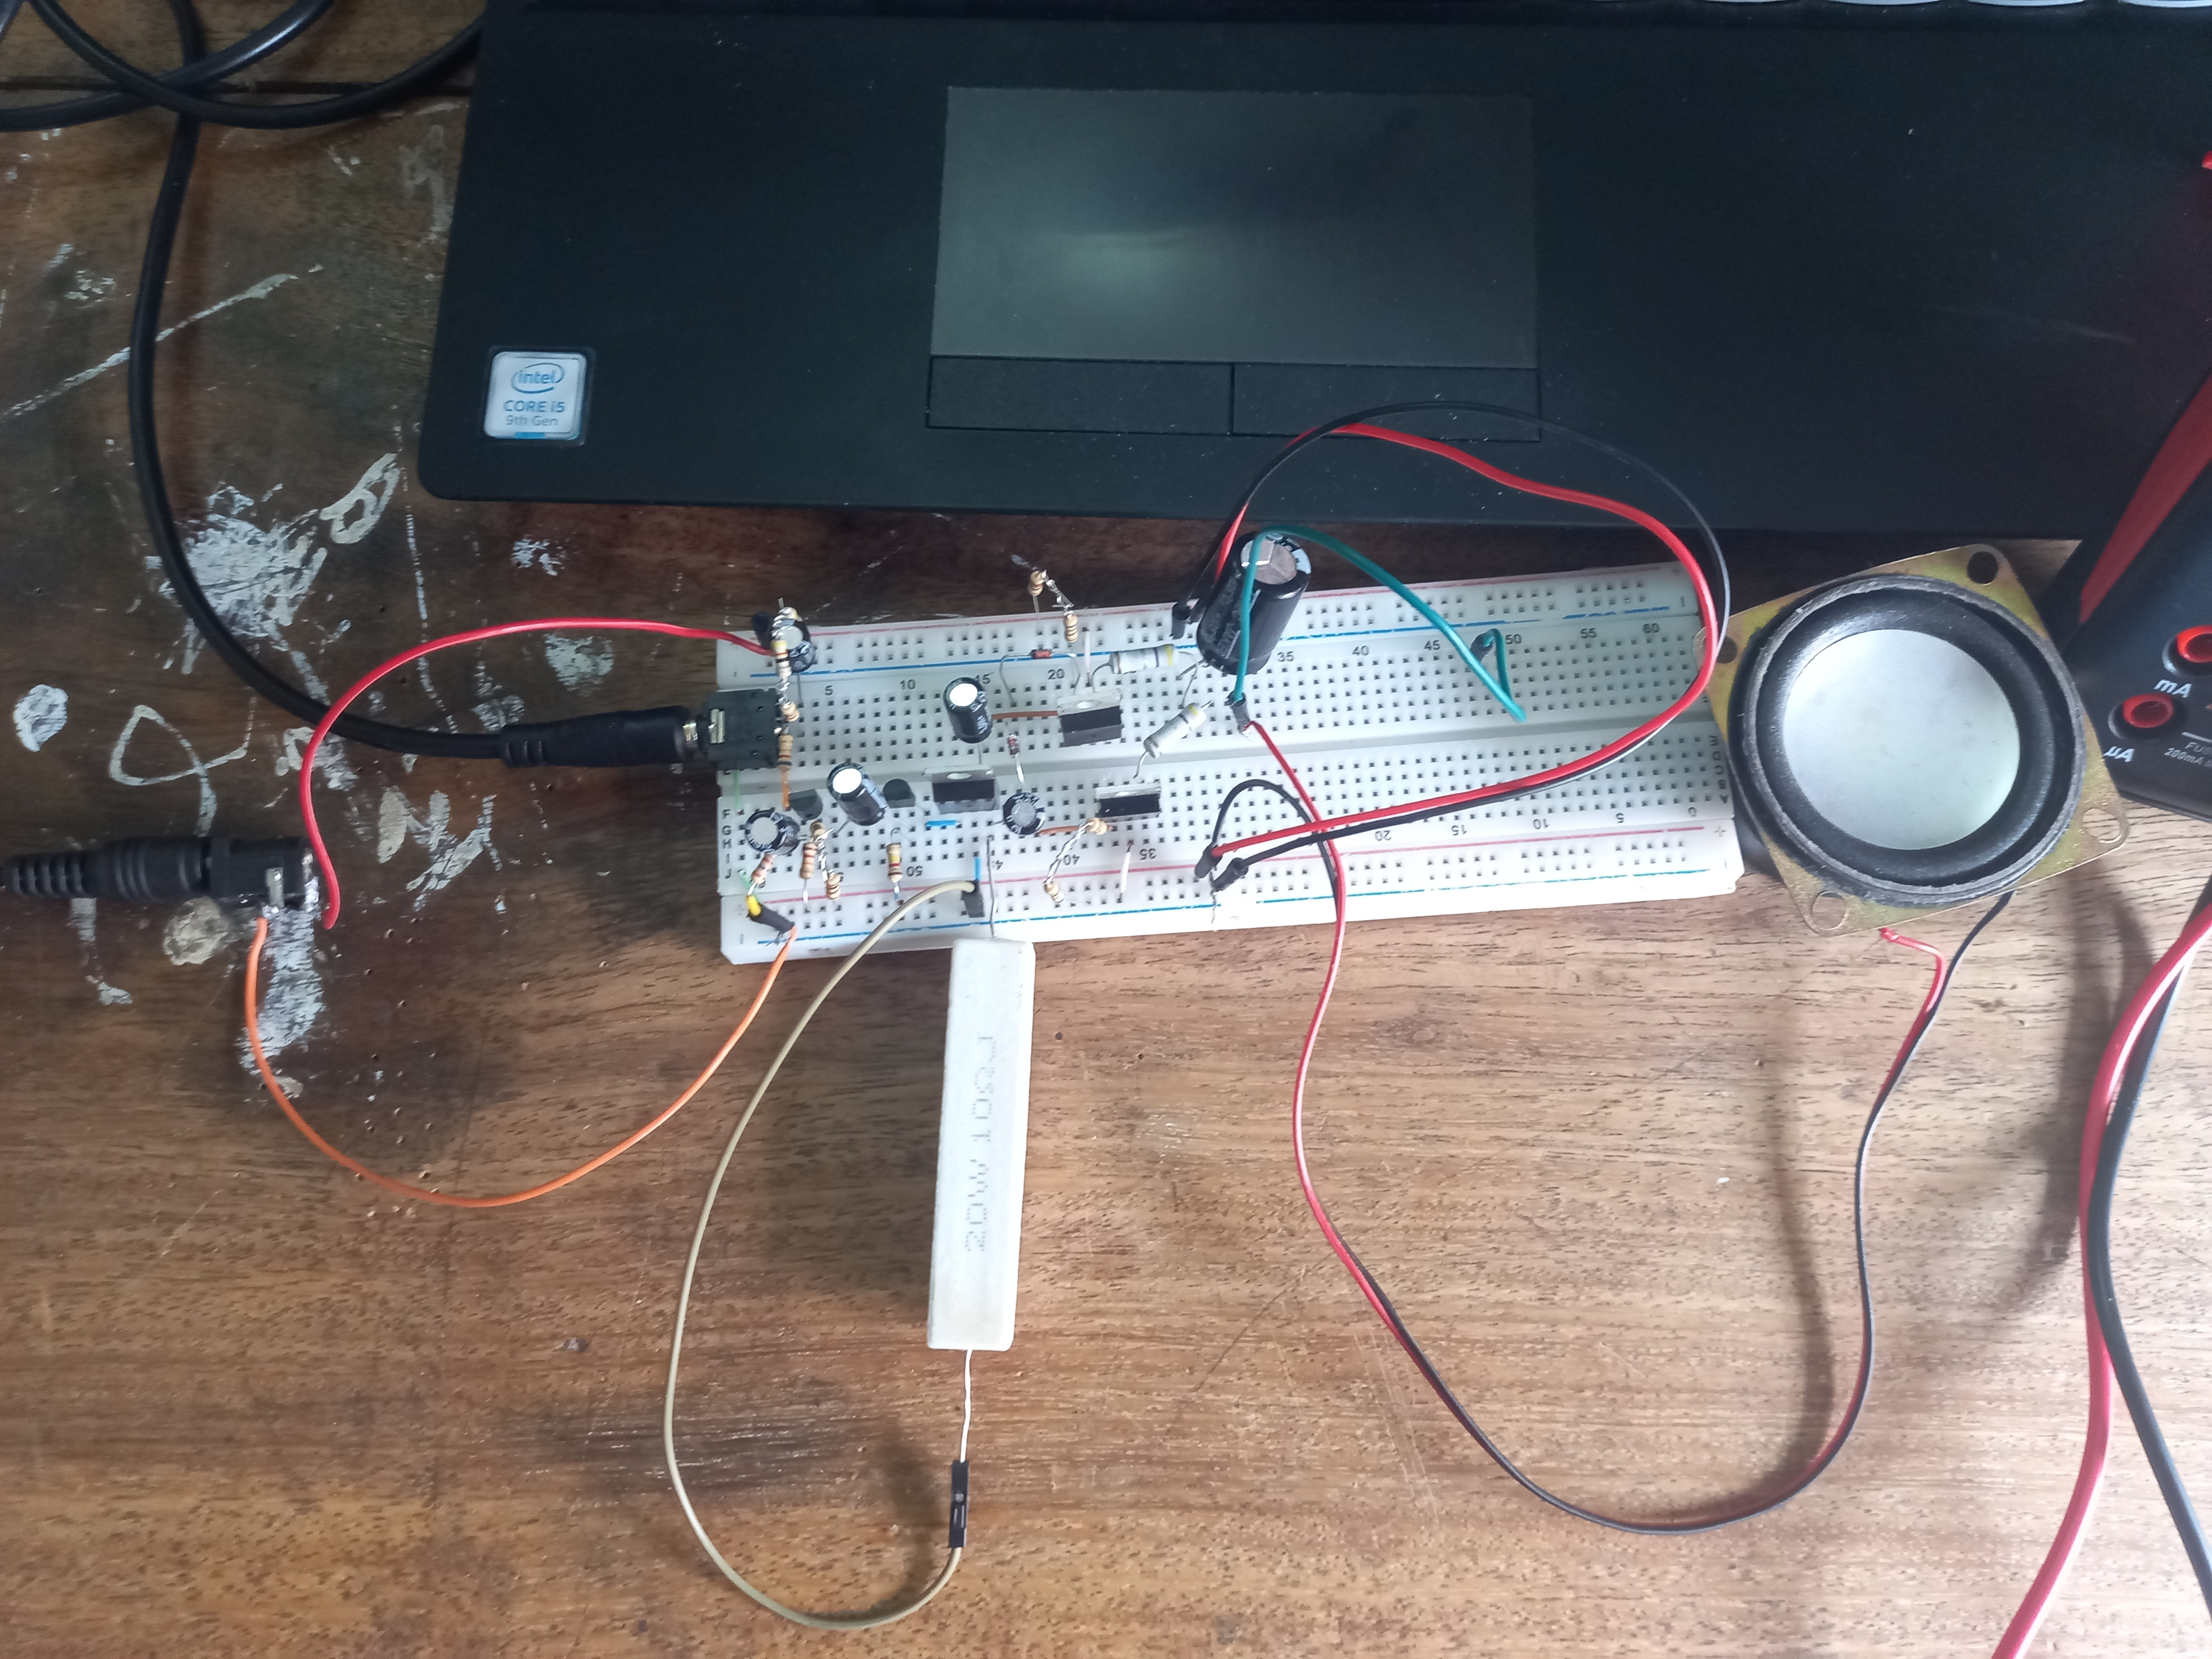
\includegraphics[height=8.75cm]{figure/breadboard.jpg}
					\end{center}
					\caption{Breadboard Testing}
					\label{refFigure15}
				\end{figure}
			\end{center}
		
		\section{Final PCB}
			Link to videos of PCB Testing: \href{https://drive.google.com/drive/folders/1nDNt05Fzzyz6RCWw_HlSfpCo1h1K3wNv?usp=sharing}{Google Drive}
			
			\begin{center}
				\begin{figure}[htp]
					\begin{center}
						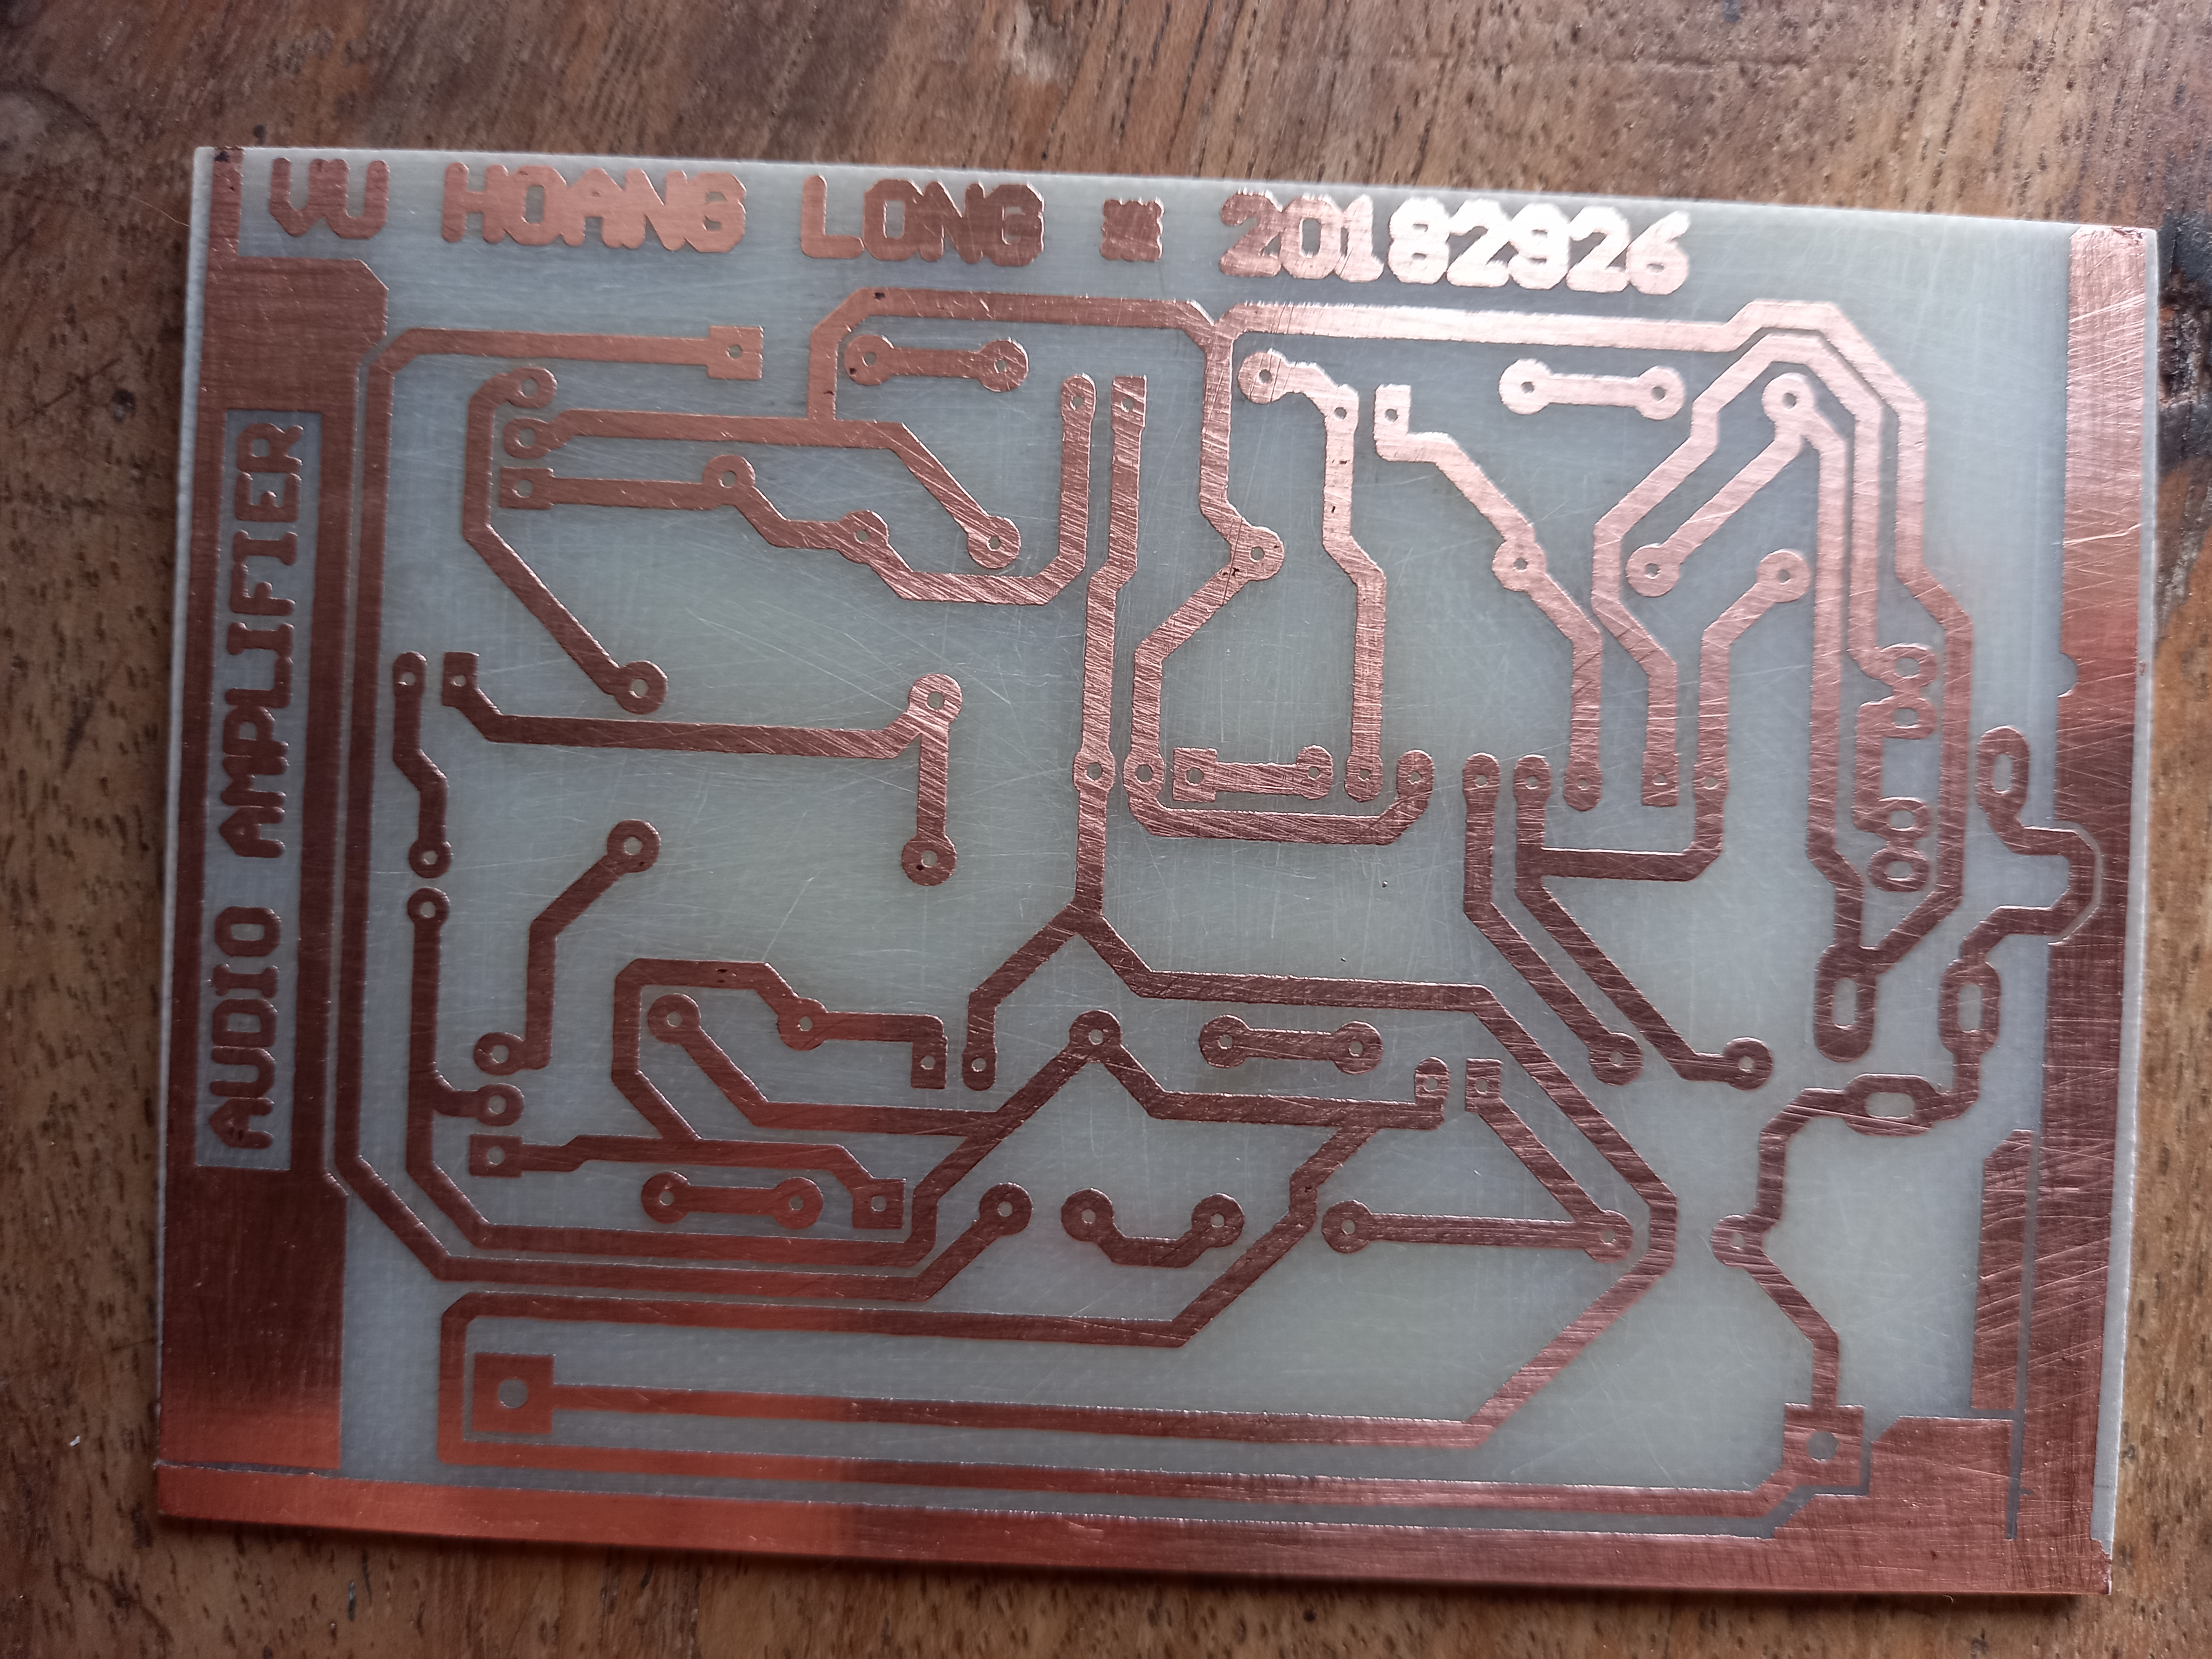
\includegraphics[height=8.75cm]{figure/printed_pcb.jpg}
					\end{center}
					\caption{PCB After Printed and Cleaned}
					\label{refFigure16}
				\end{figure}
			\end{center}
			
			\begin{center}
				\begin{figure}[htp]
					\begin{center}
						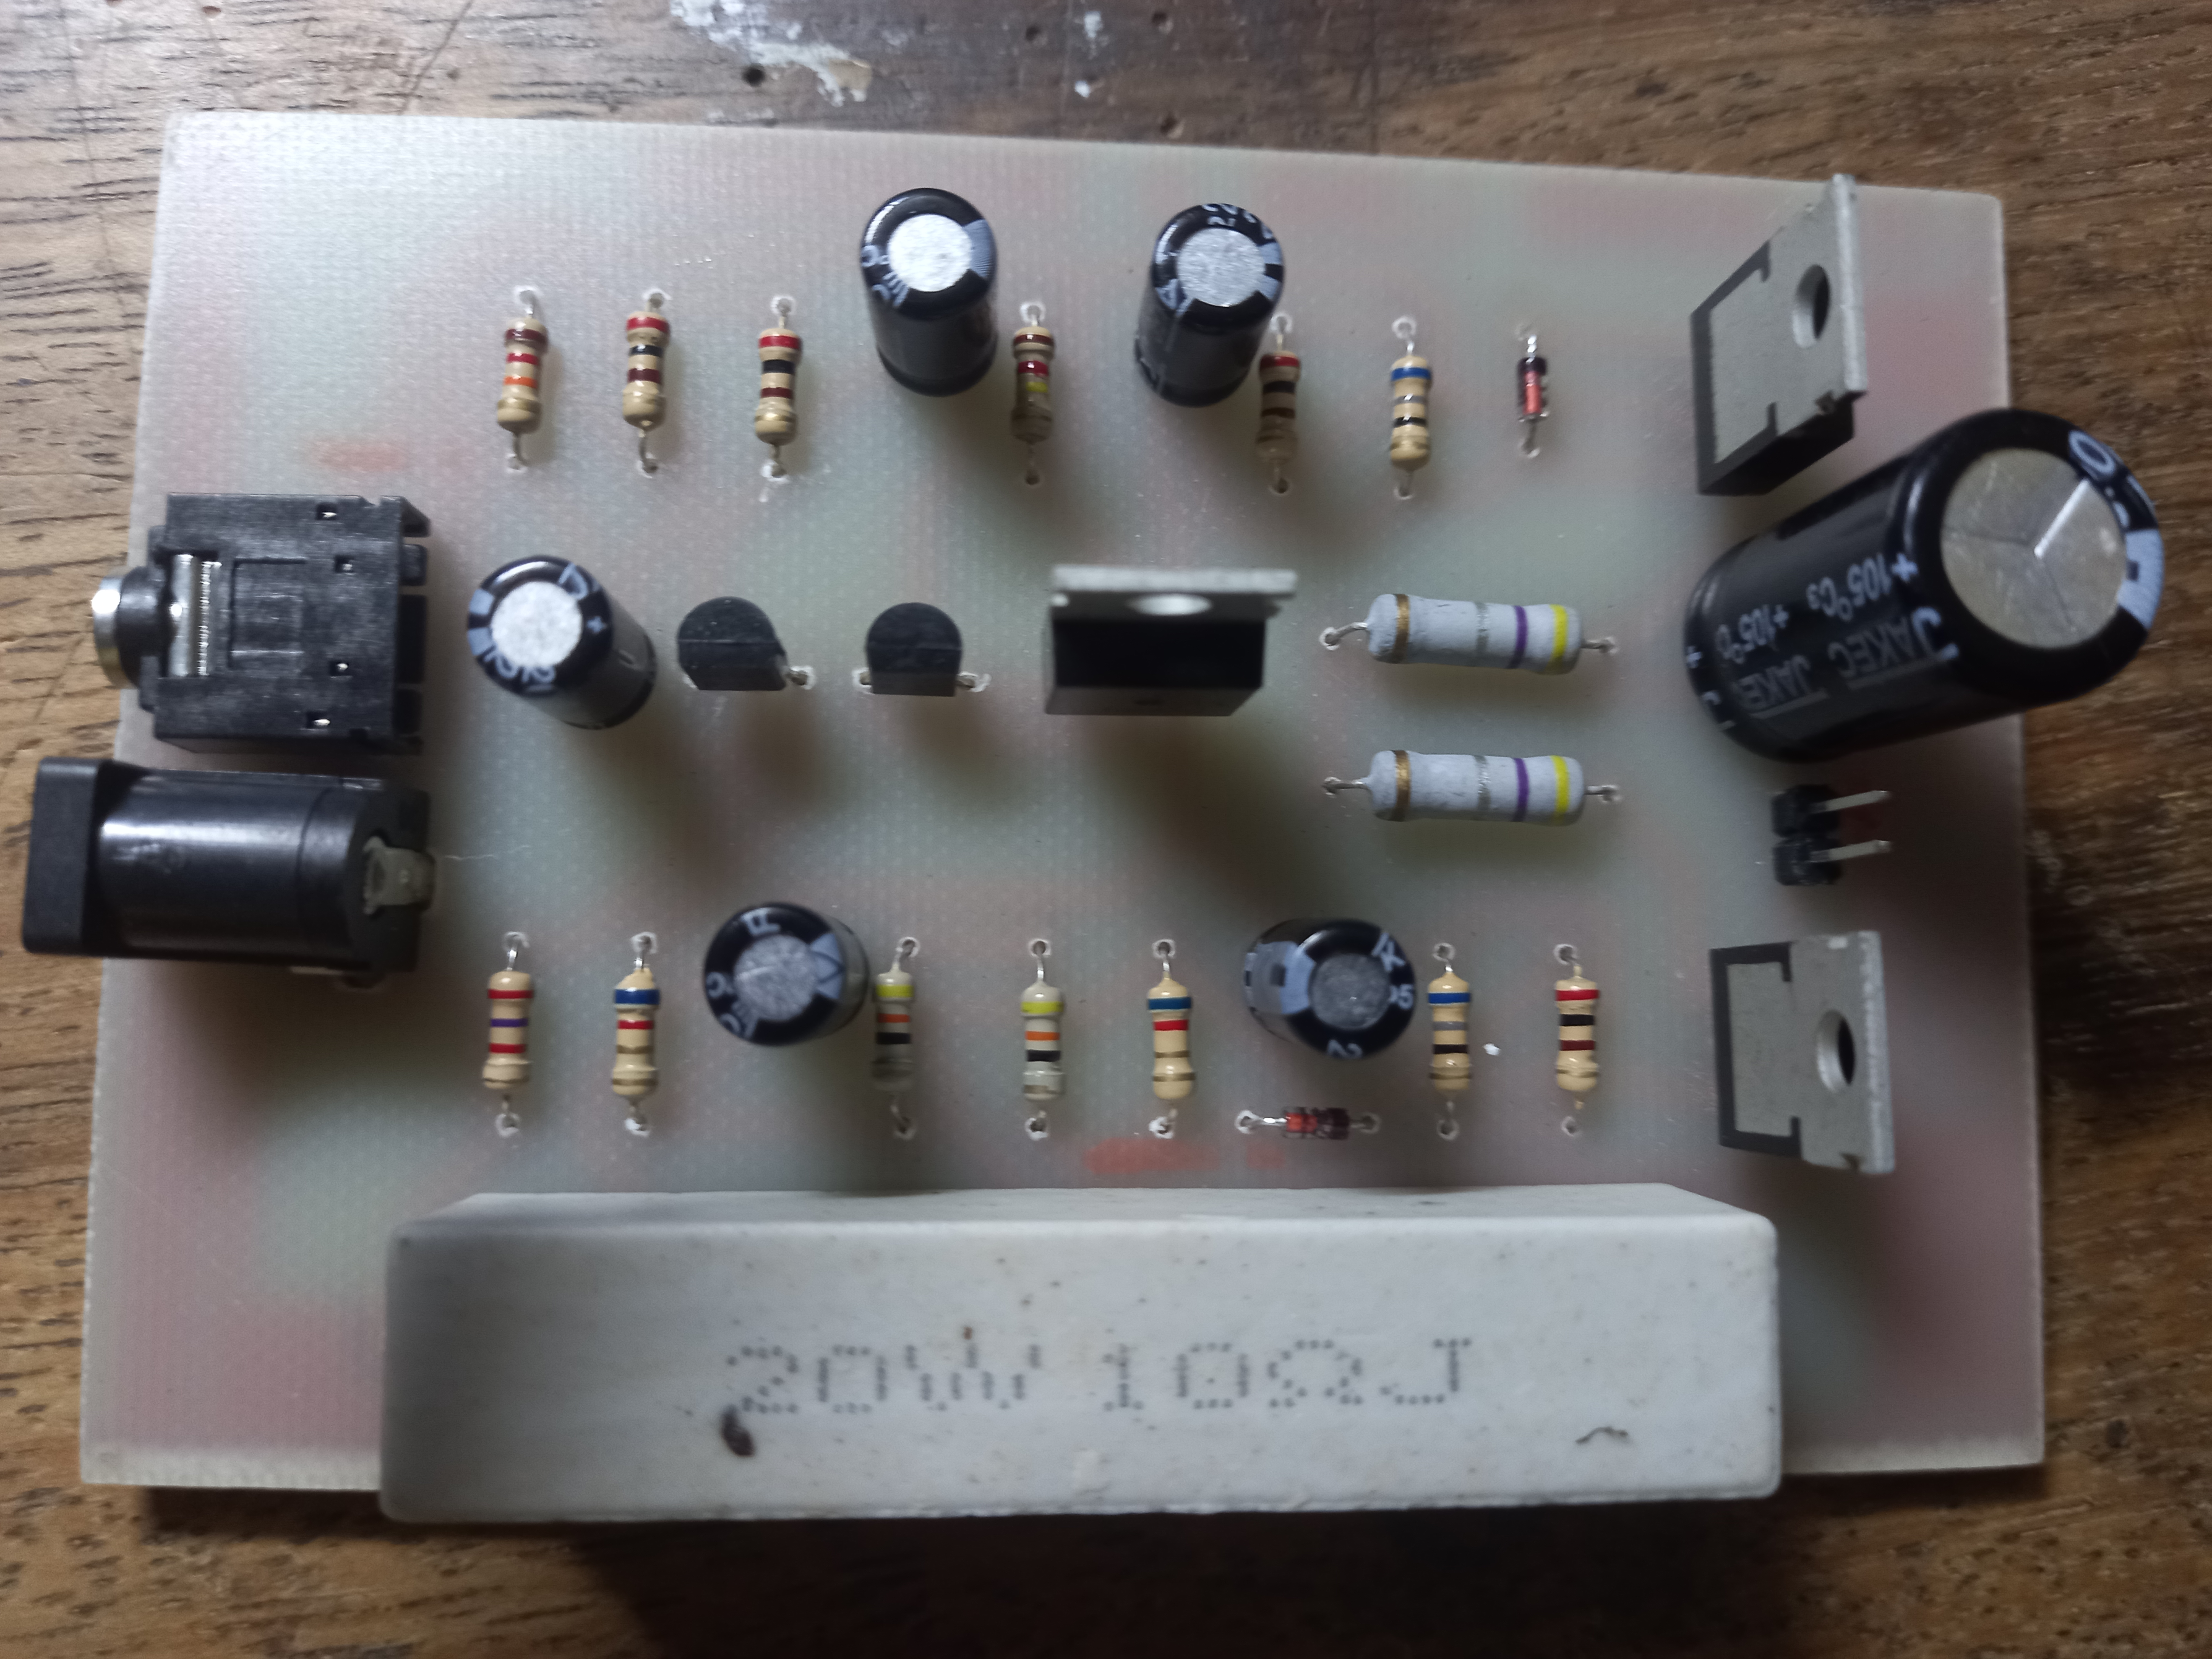
\includegraphics[height=9cm]{figure/front.jpg}
					\end{center}
					\caption{PCB Front Side}
					\label{refFigure17}
					\begin{center}
						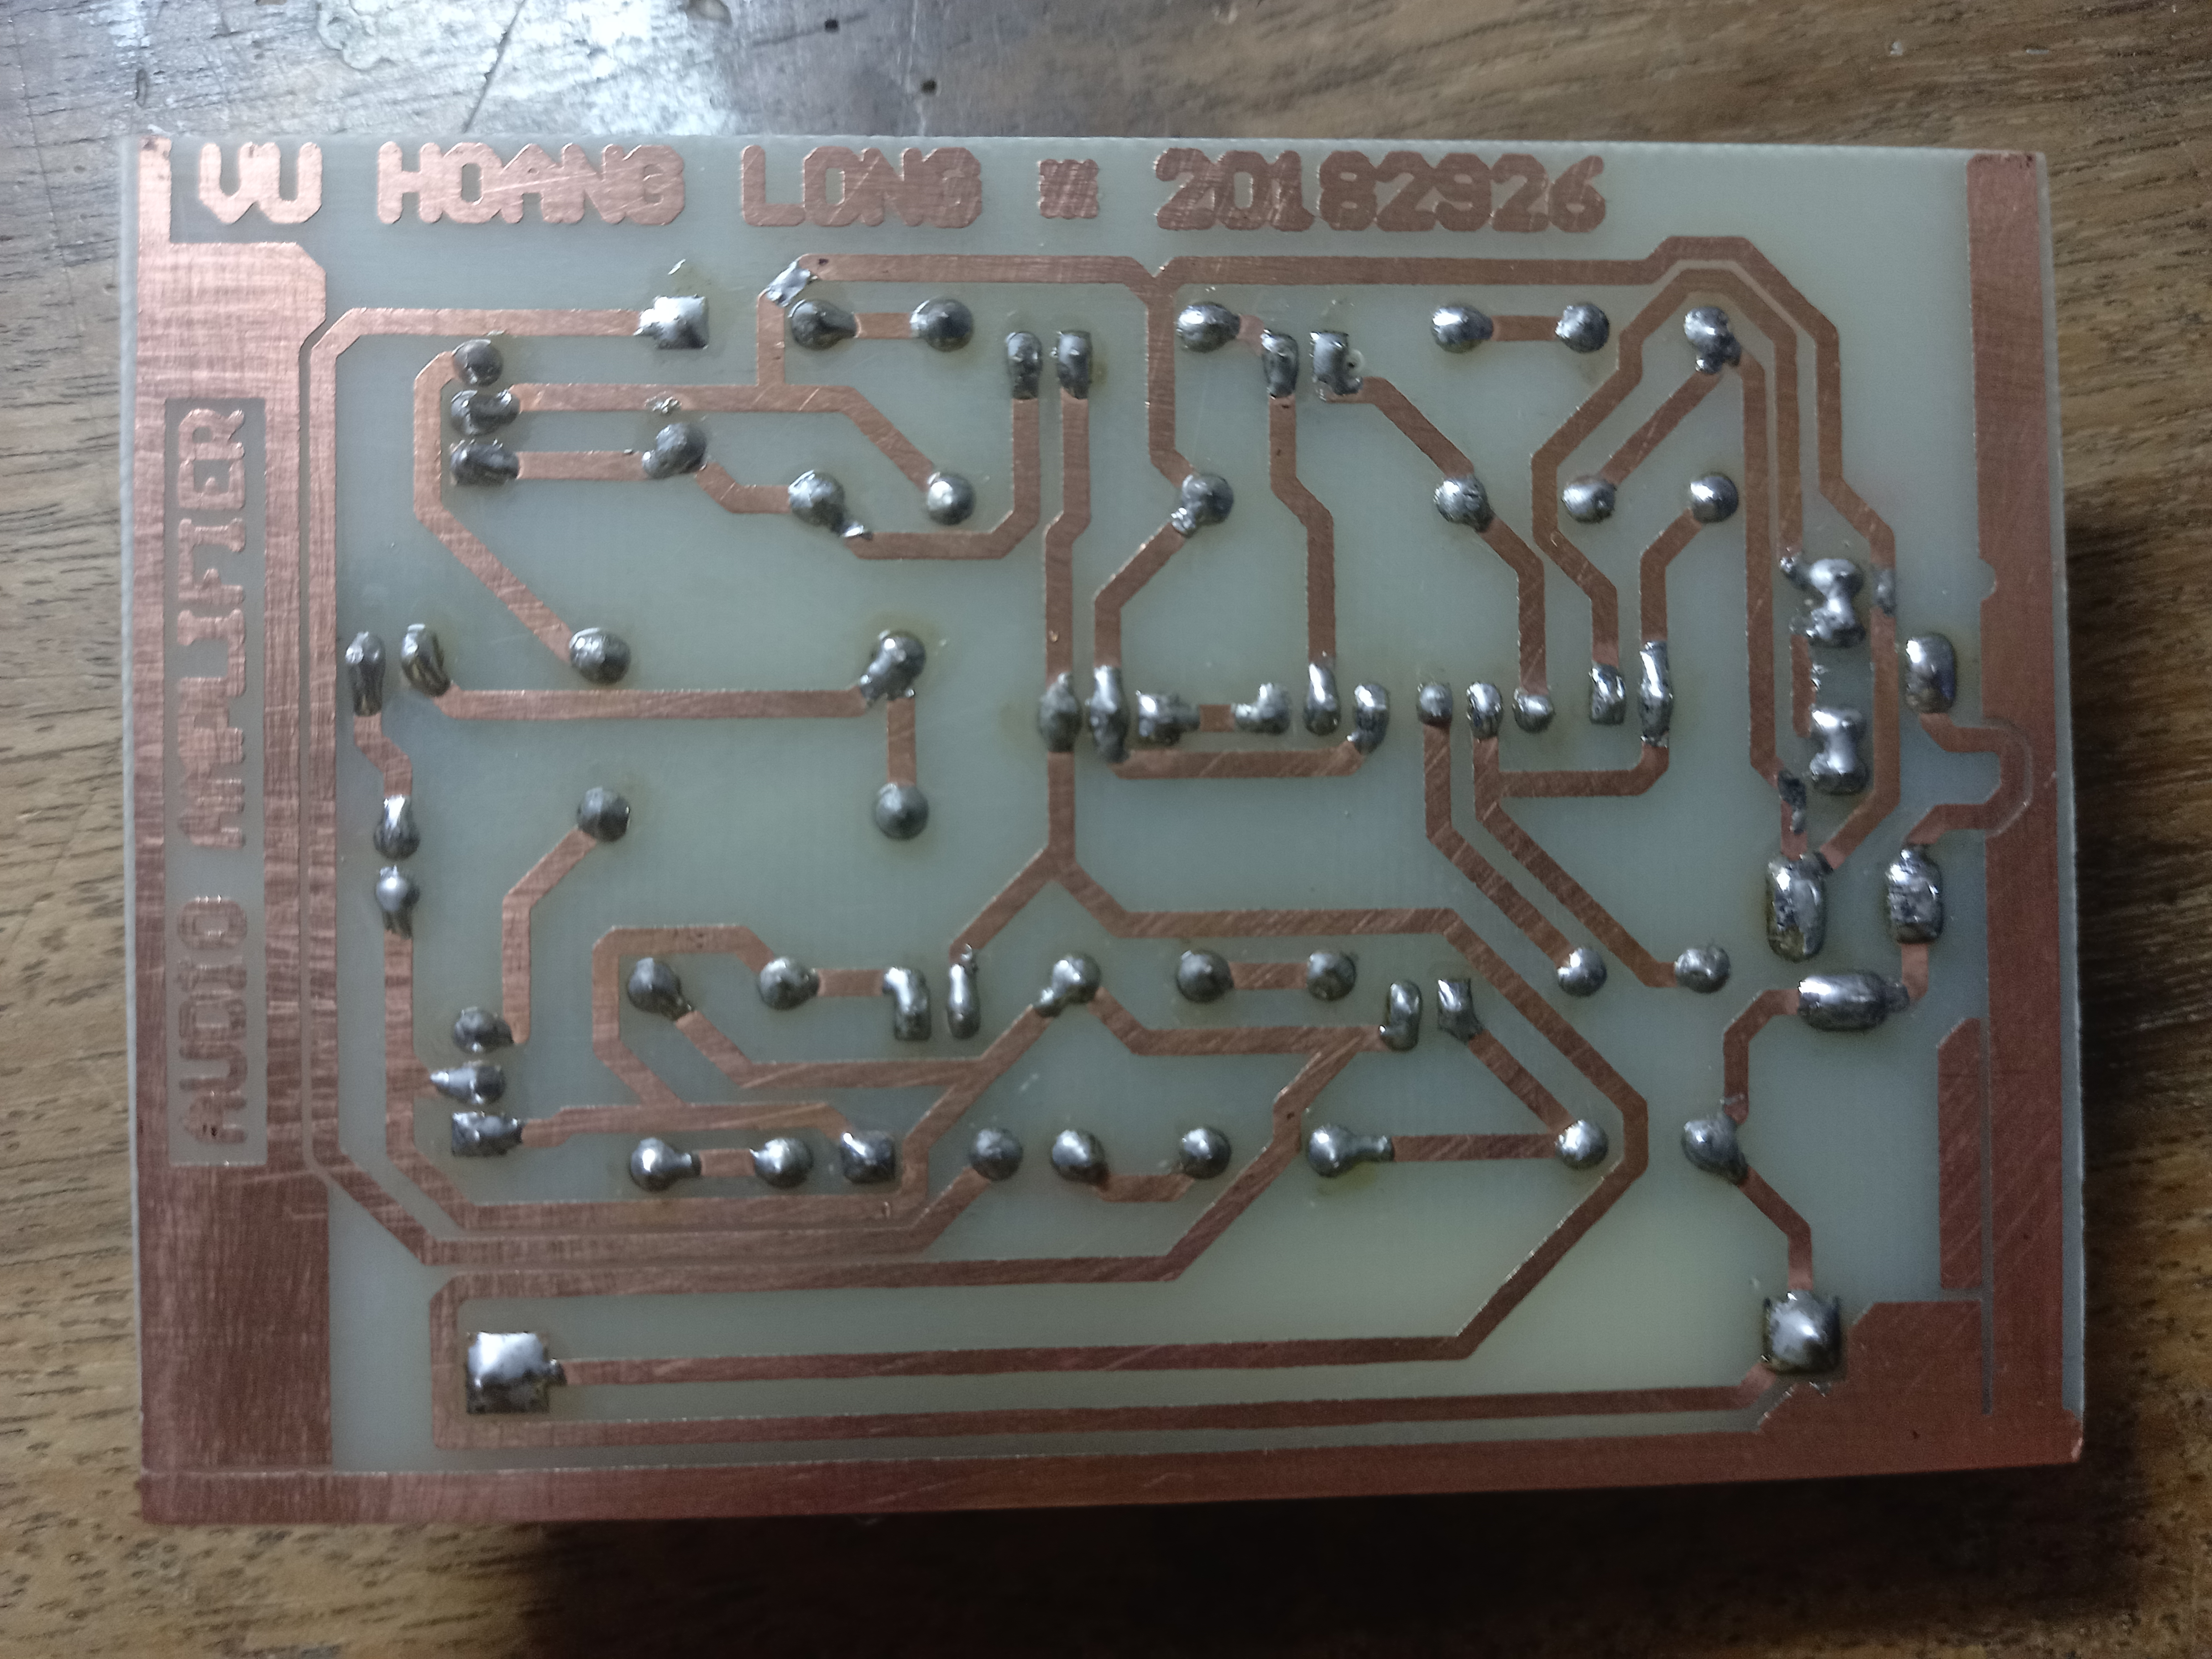
\includegraphics[height=9cm]{figure/back.jpg}
					\end{center}
					\caption{PCB Back Side}
					\label{refFigure18}
				\end{figure}
			\end{center}
		
		\newpage
		\section{Comparison}
		\begin{center}
			\begin{figure}[htp]
				\begin{center}
					\includegraphics[height=7cm]{figure/comp.png}
				\end{center}
				\caption{Comparison}
				\label{refFigure19}
			\end{figure}
		\end{center}
		The measurement video was shown in the above \href{https://drive.google.com/drive/folders/1nDNt05Fzzyz6RCWw_HlSfpCo1h1K3wNv?usp=sharing}{link}.
		
	\newpage
	\part{Conclusion}
	Comprehensively, over many times of modifying and testing, finally my calculation results match with the simulation, and then with the breadboard testing and my final PCB. Respectfully, this process and those trials considerably helps me to fill up my lack of knowledge that I can not even consider without the time for this project. Moreover, I become more familiar with the use of some very effective electronics-related software such as \textit{\textbf{Multisim}}, \textbf{\textit{Proteus}}, \textbf{\textit{Altium}}, which will be furthermore very helpful for my higher studying on the field of \textit{Electronics and Telecommunications}.
	
	Anyway, though I have worked hard and achieve a desirable accomplishment, my final project seems not to be the best one. Within the significant development of technology, everyday I see many kind of audio amplifier, or in the other word loudspeaker, with the tiny size but burly sound, also very high resolution, etc. Nevertheless whatever the world was, I have tried and will try my best to understand the basis principle of what I learn, from the simplest thing, like this project. With this way of approach, I hope those essential knowledge will help me to accelerate my further studying and career.
	
	On the way I gain my goal, without a great guide, I can not easily get it. Sincere thanks to my teacher Dr. Nguyen Vu Thang, who lighten the procedure step by step, so that I can get the right path to accomplish my project with the minimized consumed effort. Due to the limit of time, perhaps my product ends up by just a PCB, without the optimization of size and efficiency. Anyway, I am really looking forward to receive you feedback on my project so that I know my lackage and do better on the next projects. Once again, thank you very much for your devotion.
	
	\raggedleft \textit{Thank you!}
	
	
	
	
	\newpage
	\part*{Reference}
	\begin{enumerate}
		\item  Robert L. Boylestad, and  Louis Nashelsky, \textit{Electronic Devices and Circuit Theory 11th Edition}. Pearson, 2012.
		\item Pham Hong Dat, Pham Huy Thong, Nguyen Duc Thanh, Pham Thanh  Son, \textit{Bai tap lon mon hoc Dien tu tuong tu I - Mach khuech dai am thanh}. HUST, 2020.
		\item Dr.Nguyen Tien Hoa, Thesis Template. HUST, 2020.
		\item https://www.electronics-tutorials.ws/
		\item https://www.tutorialspoint.com/
		\item https://electronics.stackexchange.com/
		\item https://www.alldatasheet.com/
	\end{enumerate}
	
	
\end{document}